\section{Proposed extensions}\label{sec:extension}
%\matthias{Here we will list the things we miss in each language, and introduce possible ways of implementing them and ways to learn from eachother}
\matthias{How does ProB add HO, and what can we learn from them (and vice-versa)}
In this section, we compile a list of missing language constructs, and introduce possible ways of implementing them and ways to learn from eachother.
\subsection{Language}
HO is sometimes criticized as being to expressive.
Sometimes however, the additional structure HO exhibits allows solvers to perform better.
For example, in this case HO preserves the local coherence and independence of the different examples, a property that the solver could leverage to become more efficient.
\subsection{solver}

\begin{figure}
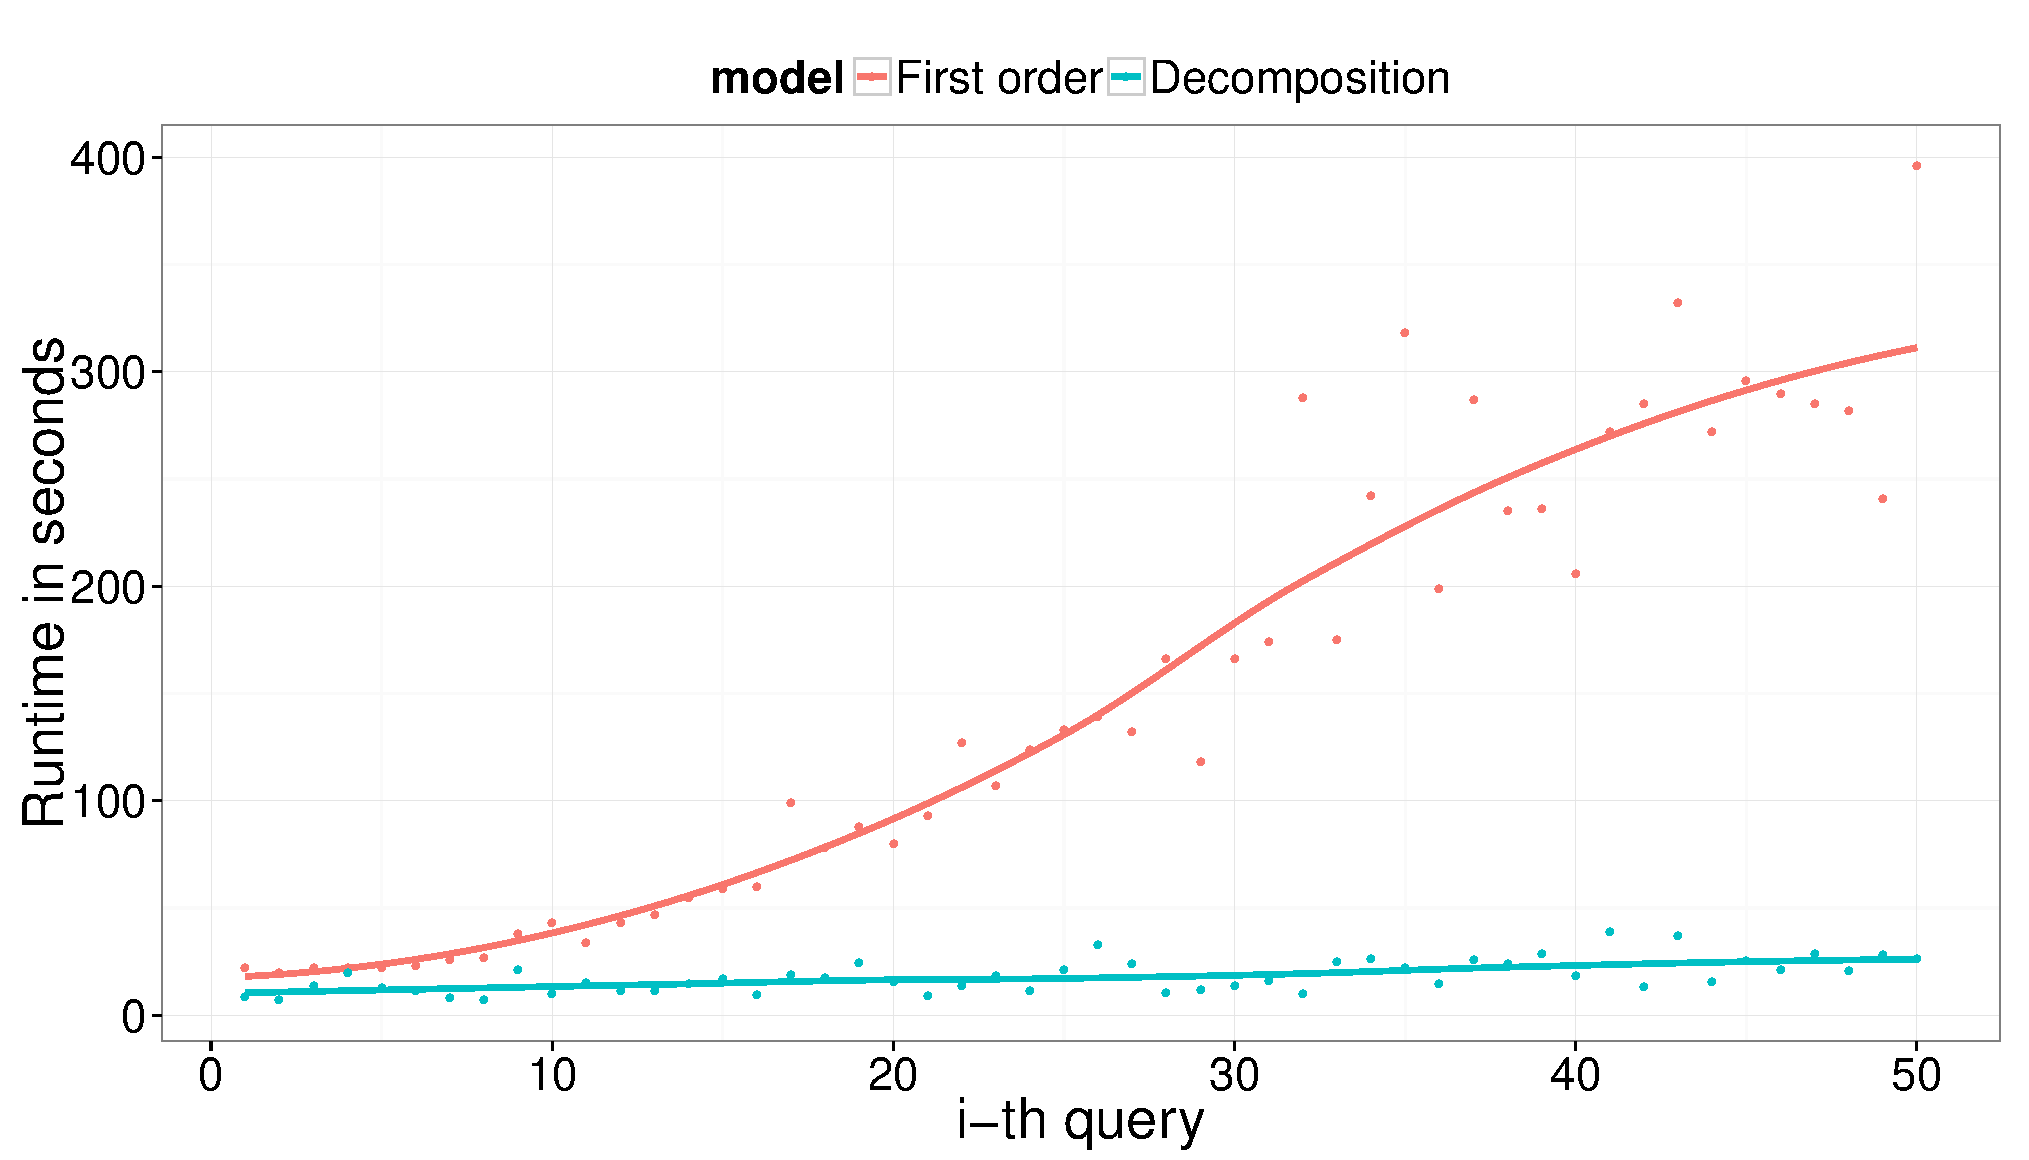
\includegraphics[width=\linewidth]{extra/figure_comparison_yoshida.pdf}
\end{figure}


\subsubsection{Oracles}
\subsubsection{Benders decomposition}

\subsection{Faithful encoding}
\matthias{In this subsection, we show a new encoding, which is not yet supported in IDP, and argue that it is more faithful to the problem with respect to the definition as given in Def~\ref{def:gm2}.}
\begin{alltt}
  homomorphism(<Edge1, Label1>, <Edge2, Label2>) \(\iff\)
      \big(\(\exists\) f: (\(\forall\) x, y : x \(\neq\) y \(\Rightarrow\) f(x) \(\neq\) f(y)) \(\wedge\)
      (\(\forall\) x, y : Edge1(x, y) \(\implies\) Edge2(f(x), f(y))) \(\wedge\)
      (\(\forall\) x : Label1(x) = Label2(f(x)))\big)

  isomorph(<Edge1, Label1>,<Edge2, Label2>) \(\iff\)
      \big(\(\exists\)f : (\(\forall\)x,y:x\(\neq\)y\(\implies\)f(x)\(\neq\)f(y)) \(\wedge\)
      (\(\forall\) x, y : Edge1(x, y) \(\iff\) Edge2(f(x), f(y))) \(\wedge\)
      (\(\forall\) x : Label1(x) = Label2(f(x)))\big).

  \textbraceleft
  reachable(x, y, Edge) \(\leftarrow\) Edge(x, y) \(\lor\) Edge(y, x).
  reachable(x, y, Edge) \(\leftarrow \exists\) : reachable(x, z, Edge) \(\wedge\) reachable(z, y, Edge).
  \textbraceright

  //\(\forall\)Pat represents quantification over a predicate Pat/2. 
  //A pattern is represented by its Edge relation. 
  \(\forall\)P : pattern(P) \(\implies\) \#\textbraceleft Pos : positive(Pos) \(\wedge\) homomorphism(P, Pos) \textbraceright \(\geq\) \(N{+}\).
  \(\forall\)P : pattern(P) \(\implies\) \#\textbraceleft Neg : negative(Neg) \(\wedge\) homomorphism(P, Neg) \textbraceright \(\leq\) \(N_\).
  \(\forall\)P,P2 : pattern(P)\(\wedge\)pattern(P2)\(\wedge\)P\(\neq\)P2 \(\iff\) \(\neg\)isomorph(P, P2).

\end{alltt}
